\documentclass[12pt, french]{article}

\usepackage{fancyhdr, fancybox, lastpage}
\usepackage[most]{tcolorbox}
\usepackage[a4paper, margin={0.3in, .75in}]{geometry}
\usepackage{wrapfig}
\pagestyle{fancy}
\renewcommand\headrulewidth{1pt}
\renewcommand\footrulewidth{1pt}
\fancyhf{}
\rhead{ \em{Zakaria Haouzan}}
\lhead[C]{\em{1ére Année Baccalauréat Sciences Expérimentales}}
\chead[C]{}
\rfoot[C]{}
\lfoot[R]{}
\cfoot[]{\em{Page \thepage / \pageref{LastPage}}}


\newtcolorbox{Box2}[2][]{
                lower separated=false,
                colback=white,
colframe=white!20!black,fonttitle=\bfseries,
colbacktitle=white!30!gray,
coltitle=black,
enhanced,
attach boxed title to top left={yshift=-0.1in,xshift=0.15in},
title=#2,#1}


\begin{document}
\begin{center}
   \shadowbox {\bf{Énergie cinétique et travail }}
\end{center}


%%_________________________Exercice ! :"_________________________Exercice
   \begin{Box2}{Exercice 1 : }
Une machine tournante a une fréquence de rotation égale à 200 tr/min. Son moment d'inertie par rapport à son axe de rotation est égal à $50 kg. m^2$ . On prendra g = 10 N/ kg.
Pour l'arrêter on exerce une force tangentielle constante de 150 N.

1. Calculer la variation d'énergie cinétique au cours du freinage.

2.Calculer le moment de la force de freinage sachant que la machine peut être assimilée à un disque de diamètre $80 cm$.

3. Calculer le nombre de tours effectués par la machine avant l'arrêt.
   \end{Box2}


%%_________________________Exercice !2 :"_________________________Exercice
\begin{Box2}{Exercice 2 : }
Un volant est constitué d'un cylindre de fonte de masse M = 1 tonne entièrement répartie sur une circonférence de rayon R = 1 m. Il tourne à une vitesse de 300 tours par minute. .

1. Calculer son moment d’inertie. $J = M.R^2$.

2. Déterminer l'énergie cinétique du volant.

3. On l'utilise pour effectuer un travail, il ralentit et ne fait plus que 120 tr / min. Calculer ce travail

4. Calculer le moment du couple s'opposant à la rotation. On prendra g = 10 N/ kg

\end{Box2}

%%_________________________Exercice ! 3:"_________________________Exercice
\begin{Box2}{Exercice 3 :}
\begin{wrapfigure}{r}{0.38\textwidth}
  \begin{center}
    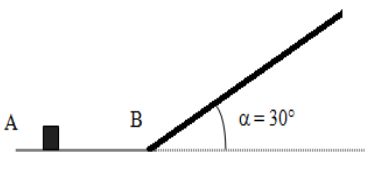
\includegraphics[width=0.38\textwidth]{./img/img00.png}
  \end{center}
\end{wrapfigure}
   Un autoporteur de masse $m = 600g$ est lancé depuis un point A avec une vitesse initiale $V_A = 6 m.s^{-1}$ sur un plan AB horizontal de longueur AB = 3 m sur lequel il glisse sans frottement, puis aborde un plan incliné BD , de
longueur $BD = 4 m$, sur lequel les frottements seront supposés négligeables.

L’autoporteur pourra être considéré comme un solide ponctuel. On prendra g = 10 N/Kg

1. Exprimer, puis calculer l’énergie cinétique de l’autoporteur en A.

2. Faire l’inventaire des forces extérieures agissant sur l’autoporteur au cours de la phase AB. Définir ces forces et les représenter sur un dessin

3.a. Donner la définition d’un système pseudo-isolé .

3.b. L’autoporteur est -il pseudo-isolé au cours de la phase AB et la phase BD ?

3.c. En déduire la vitesse du centre d’inertie du mobile en B ?

4. Soit $C_1$ un point du plan incliné tel que $BC_1 = 1 m$ Calculer le travail du poids de l’autoporteur et le travail de l’action du plan sur l’autoporteur au cours du
déplacement $BC_1$ .

   5. En appliquant le théorème de l’énergie cinétique au solide entre les instants $t_B$ et $t_{C_1}$ en déduire $V_{c_1}$

   6. Soit $C_2$ le point de rebroussement sur le plan incliné. En appliquant le théorème de l’énergie cinétique au solide entre les instants $t_B$ et $t_{C_2}$ , en déduire $BC_2$ la distance parcourue par le mobile avant de rebrousser chemin en $C_2$ .
\end{Box2}

%%_________________________Exercice 4 : _________________________Exercice
\begin{Box2}{Exercice 4 : }
Un corps solide, descend une pente
AB = 10 m en ligne droite, sans frottement,
le plan incliné fait angle $\alpha$ avec l’horizontale.
Au point A sa vitesse était nulle, à l’arrivée au point B sa vitesse est $V= 8 km.h^{-1}$ .
Calculer l’angle $\alpha$.
\end{Box2}

%%_________________________Exercice 5 : _________________________Exercice
\begin{Box2}{Exercice 5 : }
Une bille est lancée verticalement vers le haut à une altitude
h = 2,0m par rapport au sol, avec une vitesse $V_A= 10 m/s$.
On considère que le poids est la seule force appliquée à la
bille (chute libre).
On donne $g = 10 N/kg$.
Calculer en utilisant le théorème de l’énergie cinétique :

   1. La hauteur maximale atteinte par la bille.

   2. La vitesse de la bille lorsqu’elle retombe sur le sol.
\end{Box2}

\begin{Box2}{Exercice 6}
\begin{wrapfigure}{r}{0.38\textwidth}
  \begin{center}
    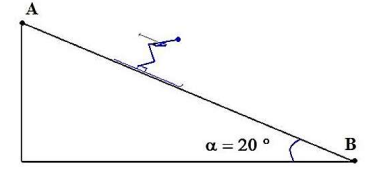
\includegraphics[width=0.38\textwidth]{./img/img02.png}
  \end{center}
\end{wrapfigure}
Un skieur descend une pente en ligne droite sur une distance AB=200m. La pente
fait un angle de $\alpha$=20° avec l’horizontale.
Au point A sa vitesse était nulle, à l’arrivée au point B sa vitesse est 30km/h. La
masse du skieur est 80 kg .
L’ensemble des forces de
frottements que subit le skieur est
équivalent à une force f parallèle
au sol mais opposée au sens du
mouvement.

   1. Représenter le skieur avec les différentes forces qui agissent sur lui et nommer ces forces.

   2. Calculer le poids du skieur et déterminer quel angle il fait avec AB.

   3. Calculer le travail du poids au cours de mouvement de A à B.

   4. Déterminer l’énergie cinétique du skieur à l’arrivée au B.

   5. Donner l’expression du théorème de l’énergie cinétique appliqué au cas de ce
skieur.


   6. Donner l’expression du travail de $\vec{f}$.

   7. Déterminer l’intensité de la force $f$.
\end{Box2}

\begin{Box2}{Exercice 7 }
\begin{wrapfigure}{r}{0.2\textwidth}
  \begin{center}
    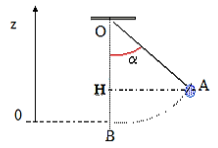
\includegraphics[width=0.2\textwidth]{./img/img03.png}
  \end{center}
\end{wrapfigure}
Une pendule est constituée d’une bille de
masse m = 200g, suspendue à un fil de
longueur L = 1,00m.

   On écarte le fil d’un angle $\alpha$ = 70° par rapport à la
verticale (position A) et on l’abandonne sans vitesse
initiale. On néglige les frottements.

   On donne g = 10 N/kg.

   1. Calculer la vitesse de la bille à son passage par la position d’équilibre (position B).
\end{Box2}

\begin{Box2}{Exercice Supplémentaire }
Brahim a lancé une bille verticalement vers le haut à une altitude h = 1,0m
avec une vitesse V=10m/s. On considère que le poids est la seule force appliquée à
la bille (chute libre).On donne g = 10N/kg.

   Calculer en utilisant le théorème de l’énergie cinétique :

   1. La hauteur maximale atteinte par la bille.

   2. La vitesse de la bille lorsqu’elle retombe sur le sol.
\end{Box2}


\vspace{2cm}
\begin{center}
   \Large{ \em{}}
\end{center}



%%_________________________Exercice 6 : _________________________Exercice
\end{document}
